% ============================================================================================
%  Betting rules that make union-of-intersections test sequences convex
%  DRAFT note -- companion to Spertus, Sridhar, and Stark, "Sequential stratified inference
%  for the mean" (arXiv:2409.06680).  Notation follows that paper.
%  Figures and tables are generated by ../code (see code/README.md); numbers quoted in the
%  text come from tables/numbers.tex, written by code/simulations.py.
% ============================================================================================
\documentclass[11pt]{article}
\usepackage[margin=1in]{geometry}
\usepackage{amsmath,amssymb,amsthm,mathtools}
\usepackage[only,llbracket,rrbracket,Lbag,Rbag]{stmaryrd}  % bags, as in the parent paper
\usepackage{graphicx,booktabs,xcolor,array}
\usepackage{microtype}
\usepackage[section]{placeins}   % keep floats within their section
\emergencystretch=1.5em
\usepackage[ruled,vlined]{algorithm2e}
\usepackage[square,authoryear]{natbib}
\usepackage[colorlinks=true,linkcolor=blue!50!black,citecolor=blue!50!black,urlcolor=blue!50!black]{hyperref}
\usepackage[capitalise,noabbrev]{cleveref}

% ---------------------------------------------------------------------------- notation
\newcommand{\bs}{\boldsymbol}
\newcommand{\E}{\mathbb{E}}
\renewcommand{\Pr}{\mathbb{P}}
\newcommand{\R}{\mathbb{R}}
\newcommand{\N}{\mathbb{N}}
\newcommand{\calC}{\mathcal{C}}
\newcommand{\calX}{\mathcal{X}}
\newcommand{\KLinf}{\mathrm{KL}_{\inf}}
\newcommand{\up}{\mathrm{UP}}
\newcommand{\mix}{\mathrm{mix}}
\newcommand{\cbar}{\bar c}
\newcommand{\conv}[1]{\breve{#1}}          % convex envelope (appendix)
\DeclareMathOperator*{\argmin}{arg\,min}
\DeclareMathOperator*{\argmax}{arg\,max}
\newcommand{\todo}[1]{{\color{red!70!black}\textsf{[#1]}}}

\theoremstyle{plain}
\newtheorem{theorem}{Theorem}
\newtheorem{proposition}[theorem]{Proposition}
\newtheorem{lemma}[theorem]{Lemma}
\newtheorem{corollary}[theorem]{Corollary}
\theoremstyle{definition}
\newtheorem{definition}[theorem]{Definition}
\newtheorem{assumption}{Assumption}
\newtheorem{example}[theorem]{Example}
\theoremstyle{remark}
\newtheorem{remark}[theorem]{Remark}

% generated by code/simulations.py -- do not edit by hand
\newcommand{\repsB}{100}
\newcommand{\repsF}{1000}
\newcommand{\repsH}{500}
\newcommand{\repsI}{300}
\newcommand{\repsE}{100}
\newcommand{\repsG}{5}
\newcommand{\grapaconvloss}{0.1}
\newcommand{\agrapaconvloss}{15.5}
\newcommand{\agrapalocalminshare}{84\%}
\newcommand{\agrapamissshare}{19\%}
\newcommand{\upKthree}{46.6}
\newcommand{\grapaKthree}{49.8}
\newcommand{\agrapaKthree}{43.6}
\newcommand{\kellyrefKthree}{49.3}
\newcommand{\taylorrefKthree}{48.5}
\newcommand{\fkellyvsagrapamin}{15\%}
\newcommand{\fkellyvsagrapamax}{19\%}
\newcommand{\fupvsagrapamin}{4\%}
\newcommand{\fupvsagrapamax}{25\%}
\newcommand{\ftaylorvskellymax}{46\%}
\newcommand{\ffixedtau}{2676}
\newcommand{\fkellytau}{42}
\newcommand{\ffixedcens}{88\%}
\newcommand{\ffixedgapcens}{100\%}
\newcommand{\fsonebest}{8}
\newcommand{\fndesigns}{10}
\newcommand{\timeKmax}{1000}
\newcommand{\timeNmax}{50000}
\newcommand{\timewfKmax}{86}
\newcommand{\timewfKhundred}{9}
\newcommand{\timecvKhundred}{204}
\newcommand{\timeupKhundred}{419}
\newcommand{\timediffmax}{4e-05}
\newcommand{\timewfbelowcv}{206}
\newcommand{\timecvfail}{12}
\newcommand{\timecvruns}{30}
\newcommand{\timecvfailflat}{12}
\newcommand{\timecvokflat}{0}
\newcommand{\timecvfailKmin}{50}
\newcommand{\hratiozero}{0.92}
\newcommand{\hratioAup}{5.4}
\newcommand{\hratioBup}{2.4}
\newcommand{\hratioAkelly}{9.1}
\newcommand{\hratioBkelly}{4.4}
\newcommand{\hratioCmax}{1.05}
\newcommand{\hstratAzero}{52}
\newcommand{\hstratAmax}{98}
\newcommand{\hunstratAmax}{525}
\newcommand{\iselgainmax}{23\%}
\newcommand{\iselgainmin}{7\%}
\newcommand{\iselmeansdiff}{3\%}
\newcommand{\iselvsoraclemax}{7\%}
\newcommand{\iselbeatoracle}{3}
\newcommand{\pstarA}{0.50}
\newcommand{\pstarB}{0.65}
\newcommand{\pstarC}{0.28}
           % key numbers from the simulations (generated)

\title{Betting rules that make union-of-intersections test sequences convex\\[2pt]
       \large Draft note}
\author{Jacob V. Spertus}
\date{\today}

\begin{document}
\maketitle

\begin{abstract}
A union-of-intersections test sequence (UI-TS) for the mean of a stratified bounded population is the minimum, over
the set $\calC$ of stratumwise null means consistent with the global null, of a product of betting test
supermartingales.  Whether that minimum can be computed depends on the bets.  We characterize the bets that make the
objective convex over $\calC$, which we call convexifying: those whose payoffs on the two extreme outcomes are
log-convex functions of the null mean.  The class is closed under products and mixtures, and it contains every bet
whose fraction of wealth wagered does not depend on the null.  It excludes truncated rules such as AGRAPA, GRAPA and
ALPHA.  Convexity costs nothing asymptotically: the growth rate of any UI-TS is limited by a least-favorable null, and
a single null-free fraction, the Kelly fraction at that null, grows as fast as betting Kelly separately at every
null.  We give three ways to choose the fraction (a predictable Kelly fraction at the estimated least-favorable null,
a Taylor approximation to it, and a universal-portfolio mixture over the fraction), compute the UI-TS by
water-filling, in time linear in the number of observations for the first two, which scales to thousands of strata,
and select strata
greedily by an upper confidence bound on the Kelly growth rate at the estimated least-favorable null, which keeps
the objective convex.
\end{abstract}

% ============================================================================================
\section{Introduction}\label{sec:intro}
% ============================================================================================

\citet{spertus2024sequential} test hypotheses about the mean of a bounded population sampled by
strata, sequentially and with finite-sample, nonparametric validity.  The global null $H_0 : \mu^\star \le \eta_0$
is written as a union of intersection hypotheses about the stratum means; each intersection hypothesis is
tested by an intersection test supermartingale (I-TSM), a product of stratumwise betting TSMs; and the global test
statistic, the union-of-intersections test sequence (UI-TS), is the smallest I-TSM over the intersection nulls in the
union.

The minimum is over a $(K-1)$-dimensional polytope, and its difficulty depends on the betting rules.  When the bets
do not depend on the null, the log~I-TSM is concave in the null, so the minimum is attained at a vertex, and the
vertices can be enumerated for up to about $16$ strata.  When the bets are inverse in the null,
$\lambda_{kt} = c_{kt}/\eta_k$, the log~I-TSM is convex and the minimum can be computed by convex optimization for
many strata \citep[Section 5]{spertus2024sequential}.  Bets that are tuned to the alternative, such as AGRAPA, are
neither; the UI-TS is then computed by partitioning the null set into bands.

This note asks how large the convex class is, whether it contains bets that are (approximately) Kelly optimal, and
how to compute and use the resulting UI-TS.  The answers are:

\begin{enumerate}
  \item \textbf{A characterization} (\cref{thm:characterization}).  A bet is convexifying if and only if its payoffs
  on the extreme outcomes, $1-\eta\lambda(\eta)$ and $1+(1-\eta)\lambda(\eta)$, are log-convex.  The class is closed under
  products and mixtures (\cref{prop:closure}).
  \item \textbf{Null-free fractions.}  Writing the bet as a fraction of wealth, $\lambda=c/\eta$, every fraction
  $c\in[0,1)$ that does not depend on the null is convexifying (\cref{cor:nullfree}).  Truncating the bet at nulls above
  the estimated mean, as AGRAPA, GRAPA and ALPHA do, is incompatible with convexity (\cref{prop:truncation}).
  \item \textbf{Convexity costs nothing asymptotically} (\cref{thm:nocost}).  For any selection rule that does not depend
  on the null, betting the Kelly fraction at the least-favorable null, one fraction per stratum, grows as fast as
  betting Kelly separately at every null, and no UI-TS grows faster.
  \item \textbf{Three strategies for the fraction} (\cref{sec:strategies}): the predictable Kelly fraction at the
  estimated least-favorable null, its Taylor approximation (the derivation behind AGRAPA, applied at one null rather
  than at every null), and a universal-portfolio mixture over the fraction.
  \item \textbf{Computation and selection.}  For all three strategies the UI-TS is a smooth convex program with one
  linear constraint, solved by one-dimensional water-filling at a cost linear in the number of observations for the
  first two (\cref{sec:waterfill}).  Selecting strata by an upper confidence bound on the Kelly growth rate at the estimated
  least-favorable null keeps the objective convex and approximates the optimal allocation (\cref{sec:selection}).
\end{enumerate}

\Cref{sec:sims} compares the strategies numerically, including with an unstratified test under perfect
stratification.  \Cref{app:convexify} sketches a way to convexify arbitrary stratumwise bets, and \cref{app:regret}
relates the mixture strategy to stratified empirical likelihood.

% ============================================================================================
\section{Setup}\label{sec:setup}
% ============================================================================================

We follow the notation of \citet{spertus2024sequential}.  The population is a tuple of $K$ bags
$\calX_{\bs N} = (\calX_k)_{k=1}^K$, $\calX_k = \Lbag x_{ki}\Rbag_{i=1}^{N_k}$, with values in $[0,1]$.
Stratum means are $\mu_k := \mu(\calX_k)$, stratum weights are $w_k := N_k/N$, and the population mean is
$\mu = \bs w \cdot \bs\mu$.  Starred quantities are the true, unknown ones.  The global null is
$H_0 : \mu^\star \le \eta_0$, and the set of intersection nulls is
\begin{equation}\label{eq:C}
\calC := \{\bs\eta \in [0,1]^K : \bs w\cdot \bs\eta = \eta_0\}.
\end{equation}

Within stratum $k$, $X_{k1}, X_{k2},\ldots$ are the draws in order, and after $t$ draws overall, $T_k(t)$ have come
from stratum $k$.  Throughout, sampling is with replacement; \cref{sec:discussion} comments on sampling without
replacement.  A betting TSM for the stratum null $\mu_k\le\eta_k$ is
\begin{equation}\label{eq:betting-tsm}
M_{kt}(\eta_k) := \prod_{i=1}^{T_k(t)} \bigl[1 + \lambda_{ki}(\eta_k)\,(X_{ki}-\eta_k)\bigr],
\qquad \lambda_{ki}(\eta_k) \in [0, 1/\eta_k),
\end{equation}
where $\lambda_{ki}(\cdot)$ is \emph{predictable}: it may depend on all draws made before $X_{ki}$, from any stratum.
The I-TSM is $M_t(\bs\eta) := \prod_{k=1}^K M_{kt}(\eta_k)$.  \citet[Section 4]{spertus2024sequential} define the
UI-TS as $\min_{\bs\eta\in\calC}\max_{j\le t}M_j(\bs\eta)$.  We take the running maximum outside the minimum instead:
\begin{equation}\label{eq:uits}
M_t := \max_{j\le t}\,\min_{\bs\eta\in\calC} M_j(\bs\eta).
\end{equation}
This is never larger than the original definition, needs only one minimization per time step, and is valid for the
same reason: under $H_0$ some intersection null in $\calC$ is true (raise the true stratum means until their weighted
mean reaches $\eta_0$), \eqref{eq:uits} is at most the running maximum of the I-TSM at that null, and that I-TSM is a
TSM, so by Ville's inequality \citep{ville1939etude} the probability that $M_t$ ever reaches $1/\alpha$ is at most
$\alpha$.

We restrict attention to the setting in which the I-TSM decomposes across strata.

\begin{assumption}[Stratumwise bets, $\eta$-oblivious selection]\label{ass:separable}
The bet $\lambda_{ki}$ depends on $\bs\eta$ only through $\eta_k$, and the selections $T_k(t)$ do not depend on $\bs\eta$.
\end{assumption}

Under \cref{ass:separable}, with $L_{kt}(\eta_k) := \log M_{kt}(\eta_k)$,
\begin{equation}\label{eq:separable}
\log M_t(\bs\eta) = \sum_{k=1}^K L_{kt}(\eta_k),
\end{equation}
so the shape of the UI-TS objective is determined by the shapes of $K$ univariate functions.  All the betting rules
in \citet{spertus2024sequential} satisfy the first half of \cref{ass:separable}.  The second half allows selection
rules that use the data, including the current minimizer of the objective, but not rules whose choice depends on the
null at which the I-TSM is being evaluated.

It is convenient to write a bet in terms of the \emph{fraction of wealth wagered}, $c := \eta\lambda \in [0,1)$.  The
one-step wealth factor is then
\begin{equation}\label{eq:fraction}
1 + \lambda(\eta)(x-\eta) = 1 - c(\eta) + c(\eta)\,\frac{x}{\eta},
\end{equation}
a portfolio that keeps $1-c$ in cash and puts $c$ in an asset whose return is $x/\eta$.

% ============================================================================================
\section{Which bets make the UI-TS convex?}\label{sec:convex}
% ============================================================================================

\begin{definition}[Convexifying betting rules]\label{def:rules}
A \emph{betting rule} is a function $\lambda:(0,1)\to[0,\infty)$ with $\lambda(\eta) < 1/\eta$.  It is \emph{convexifying}
(resp.\ \emph{concavifying}) if $\eta\mapsto \log[1+\lambda(\eta)(x-\eta)]$ is convex (resp.\ concave) on $(0,1)$ for
every $x\in[0,1]$.  A betting TSM is convexifying (resp.\ concavifying) if $\eta\mapsto\log M_{kt}(\eta)$ is convex
(resp.\ concave) for every data sequence.
\end{definition}

The definition requires that convexity holds for every realizable sequence, not just in expectation.
We further define the \emph{extreme payoffs} of a betting rule as
\[
g_0(\eta) := 1-\eta\lambda(\eta) = 1-c(\eta), \qquad g_1(\eta) := 1+(1-\eta)\lambda(\eta),
\]
the wealth factors on the worst and best possible outcomes, $x=0$ and $x=1$.
The key observation is that the wealth factor is affine in the outcome:
\begin{equation}\label{eq:affine-in-x}
1+\lambda(\eta)(x-\eta) = (1-x)\,g_0(\eta) + x\,g_1(\eta), \qquad x\in[0,1].
\end{equation}

\begin{theorem}[Characterization]\label{thm:characterization}
A betting rule is convexifying if and only if its extreme payoffs $g_0$ and $g_1$ are log-convex on $(0,1)$.
\end{theorem}

\begin{proof}
Necessity: take $x=0$ and $x=1$ in \cref{def:rules}.  Sufficiency: $g_0 > 0$ because $\lambda<1/\eta$, and
$g_1\ge1$.  By \eqref{eq:affine-in-x}, the wealth factor is a nonnegative combination of $g_0$ and $g_1$, and sums of
log-convex functions are log-convex \citep[Section 3.5.2]{boyd2004convex}.
\end{proof}

There is no analogous characterization of concavifying rules, because sums of log-concave functions need not be
log-concave.  A sufficient condition is that $g_0$ and $g_1$ are concave: then the factor is concave by
\eqref{eq:affine-in-x}, hence log-concave.  Fixed bets, for which $g_0$ and $g_1$ are affine, satisfy it.

\begin{corollary}[Convex UI-TS]\label{cor:convex-uits}
Under \cref{ass:separable}, if every $\lambda_{ki}$ is convexifying (for every realization of the past data),
then each $L_{kt}$ is convex, and so is $\bs\eta\mapsto\log M_t(\bs\eta)$.  Each minimum in the UI-TS \eqref{eq:uits}
is then the value of a convex program.
\end{corollary}

\begin{proof}
$L_{kt}$ is a sum of convex functions, and \eqref{eq:separable} is a sum of convex functions of different coordinates.
\end{proof}

\begin{proposition}[Closure]\label{prop:closure}
Fix a stratum.  (i) If each $\lambda_i$ is convexifying, $\eta\mapsto\prod_i[1+\lambda_i(\eta)(X_i-\eta)]$ is
log-convex.  (ii) Let $\{M^{(\theta)}_t(\eta)\}_{\theta\in\Theta}$ be convexifying betting TSMs for $\mu_k\le\eta$,
and let $\pi$ be a probability measure on $\Theta$ that does not depend on the data or on $\eta$.
Then the mixture $M^{\mix}_t(\eta) := \int M^{(\theta)}_t(\eta)\,\pi(d\theta)$ is a convexifying betting TSM for
$\mu_k\le\eta$.
\end{proposition}

\begin{proof}
(i) Products of log-convex functions are log-convex.  (ii) Sums and integrals of log-convex functions are
log-convex \citep[Section 3.5.2]{boyd2004convex}; a mixture of TSMs with a fixed mixing measure is a TSM by
Fubini's theorem, and it is a betting TSM whose bets are the wealth-weighted averages of the component bets.
\end{proof}

Those averaged bets need not be convexifying step by step; only the cumulative wealth needs to be log-convex, and
mixing guarantees that.

\subsection{Examples}\label{sec:examples}

\begin{corollary}[Null-free fractions are convexifying]\label{cor:nullfree}
If the fraction $c_{ki}\in[0,1)$ is predictable and does not depend on $\eta$, the bet $\lambda_{ki}(\eta)=c_{ki}/\eta$ is
convexifying.
\end{corollary}

\begin{proof}
$g_0 = 1-c_{ki}$ is constant and $g_1 = (1-c_{ki}) + c_{ki}/\eta$ is a sum of log-convex functions.
\end{proof}

The fraction may depend on past data from every stratum, so long as it does not depend on the null at which the I-TSM
is evaluated.  The inverse bets of \citet{spertus2024sequential} are an instance.  The convexifying class is larger
than this, as the next example shows, but null-free fractions are the part of it that is easy to use.

\begin{example}[Kelly for binary outcomes]\label{ex:binary}
If $X\sim\mathrm{Bernoulli}(p)$ with $p>\eta$, the Kelly bet \citep{kelly1956new} is
$\lambda^\star(\eta) = (p-\eta)/[\eta(1-\eta)]$, and
\[
g_0(\eta) = \frac{1-p}{1-\eta}, \qquad g_1(\eta) = \frac{p}{\eta}:
\]
the Bernoulli likelihood ratio.  Both are log-convex, so the Kelly rule for binary data is convexifying on $(0,p)$
even though its fraction $c^\star(\eta) = (p-\eta)/(1-\eta)$ depends on $\eta$.  It must be truncated at $\eta = p$ to remain
a valid bet for the composite null, and that truncation is what takes it out of the class (\cref{prop:truncation}).
\end{example}

\begin{example}[Hindsight Kelly and empirical likelihood]\label{ex:el}
For observations $x_1,\ldots,x_n$, let
\begin{equation}\label{eq:el}
\ell_n(\eta) := \sup_{\lambda\in[0,1/\eta]}\sum_{i=1}^n\log[1+\lambda(x_i-\eta)]
            = \sup_{c\in[0,1]}\sum_{i=1}^n\log\Bigl[1-c+c\,\frac{x_i}{\eta}\Bigr],
\end{equation}
the log-wealth of the best constant bet in hindsight.  This is the betting form of the one-sided log
empirical-likelihood ratio for the mean \citep{owen1988empirical}; the two coincide unless the constraint
$\lambda\le1/\eta$ binds.  For each fixed $c$ the summand is log-convex in $\eta$ (\cref{cor:nullfree}), and a pointwise
supremum of convex functions is convex, so $\ell_n$ is convex.  It is not a valid TSM, because the bet is chosen in
hindsight, but it is the benchmark that predictable rules try to track.
\end{example}

\begin{example}[Expected Kelly growth]\label{ex:klinf}
For a distribution $F$ on $[0,1]$, the Kelly growth rate $\KLinf(F,\eta) := \sup_{\lambda\in[0,1/\eta]}
\E_F\log[1+\lambda(X-\eta)]$ \citep{honda2010asymptotically} is convex in $\eta$, by the argument of
\cref{ex:el} with the empirical distribution replaced by $F$.  So the Kelly-optimal I-TSM is convex in expectation
under any alternative.  It is \emph{not} convex outcome by outcome: \cref{fig:kelly} shows that, for $F$ uniform on
$[0,1]$, the factor $\log[1+\lambda^\star(\eta)(x-\eta)]$ is concave on part of $(0,\mu)$ when $x$ is small.
\end{example}

\begin{figure}[t]
  \centering
  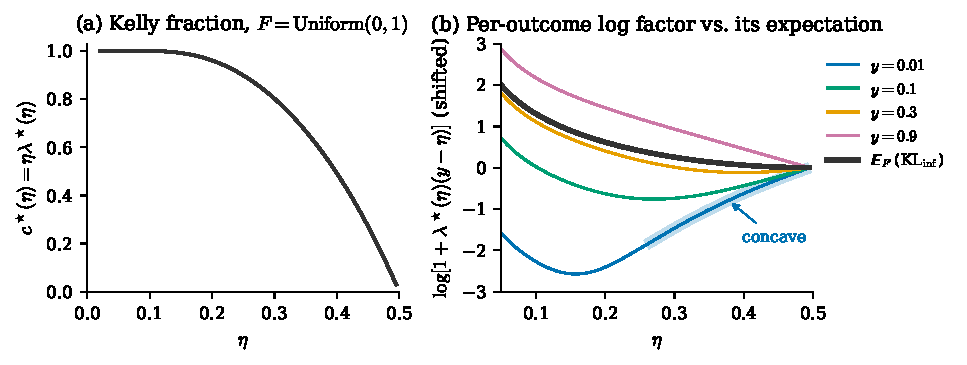
\includegraphics[width=\textwidth]{figures/fig_kelly_known.pdf}
  \caption{Kelly-optimal bets for a known alternative $F=\mathrm{Uniform}(0,1)$.  (a) The Kelly fraction
  $c^\star(\eta)=\eta\lambda^\star(\eta)$: all-in for small $\eta$, decreasing to $0$ at $\eta=\mu=1/2$.  (b) The log
  wealth factor for four outcomes (thin), shifted to $0$ at $\eta=\mu$, and its expectation, the growth rate
  $\KLinf(F,\eta)$ (thick).  The expectation is convex; the factor for outcome $0.01$ is concave on the shaded segment.}
  \label{fig:kelly}
\end{figure}

\subsection{Obstructions}\label{sec:obstructions}

The next result explains why almost every adaptive betting rule in use falls outside the convexifying class.

\begin{proposition}[Truncation is incompatible with convexity]\label{prop:truncation}
Let $\lambda$ be a convexifying rule with fraction $c(\eta)=\eta\lambda(\eta)$.  Then either $c\equiv0$ on $(0,1)$, or
$c(\eta)>0$ for every $\eta\in(0,1)$.
\end{proposition}

\begin{proof}
By \cref{thm:characterization}, $f := \log g_0 = \log(1-c)$ is convex on $(0,1)$, and $f\le0$.  Suppose $c(\eta_1)=0$
for some $\eta_1\in(0,1)$, so $f(\eta_1)=0=\max f$.  For any $\eta<\eta_1<\eta'$, write $\eta_1=\theta\eta+(1-\theta)\eta'$;
convexity gives $0=f(\eta_1)\le\theta f(\eta)+(1-\theta)f(\eta')\le0$, so $f(\eta)=f(\eta')=0$.  Hence $f\equiv0$ and
$c\equiv0$.
\end{proof}

Most adaptive rules stop betting on nulls that are above an estimate of the mean, because a positive bet there has
negative expected log-growth.  AGRAPA \citep{waudbysmith2024estimating} sets $\lambda=0$ when
$\eta\ge\hat\mu_{k(t-1)}$; GRAPA \citep{kumon2011sequential, waudbysmith2024estimating}, which maximizes the past
wealth separately at every $\eta$, does the same when the past mean is below $\eta$; and so does the truncated Kelly
rule of \cref{ex:binary}.  By \cref{prop:truncation} none of these rules is convexifying.  The failure is concrete:
each observation with $X_{kt}<\hat\mu_{k(t-1)}$ contributes a concave kink at $\eta_k=\hat\mu_{k(t-1)}$.  The
shrink-truncated Bernoulli bet (ST-Bern, from ALPHA; \citealp{stark2023alpha}) avoids zero bets by truncating its
estimate of the mean above $\eta$, but on the truncated branch its fraction is $c=\epsilon_t/(1-\eta)$, for which
$\log g_0(\eta)=\log(1-\eta-\epsilon_t)-\log(1-\eta)$ is concave.

AGRAPA also fails for a second reason that matters more in practice.  Its bet
$(\hat\mu-\eta)/[\hat\sigma^2+(\hat\mu-\eta)^2]$ is maximized at $\hat\mu-\eta=\hat\sigma$ and then \emph{decreases} as
$\eta$ moves further below $\hat\mu$, so AGRAPA bets less on nulls that are further from the estimate
(\cref{fig:anatomy}d).  Its log-wealth therefore flattens out, and is concave, far from $\hat\mu$, while the
hindsight-Kelly log-wealth $\ell_n$ grows without bound as $\eta\to0$ (\cref{fig:anatomy}a,b).  When the stratum means
differ, the AGRAPA objective along $\calC$ can then have a second local minimum (\cref{fig:anatomy}c): this happened in
\agrapalocalminshare{} of \repsE{} runs with $K=2$, $\bs\mu=(0.52,0.90)$ and $n_k=150$, and with $K=3$ a local search from
the center of $\calC$ missed AGRAPA's global minimum by more than $0.05$ in \agrapamissshare{} of runs
(\cref{sec:sims}).

% ============================================================================================
\section{Betting fractions that do not depend on the null}\label{sec:fractions}
% ============================================================================================

By \cref{cor:nullfree}, any predictable fraction $c_{kt}\in[0,1)$ that does not depend on the null yields a
convexifying bet $\lambda_{kt}(\eta_k)=c_{kt}/\eta_k$, and a convex UI-TS.  This section asks how to choose the fraction,
how to compute the UI-TS, and how to choose which stratum to sample.

The obvious idea, maximizing the past wealth over $c$ separately at each null, gives back GRAPA, which is not
convexifying (\cref{prop:truncation}): the maximizing fraction is zero at nulls above the past mean.  The
optimization has to be done once, at a single reference null, and the resulting fraction applied at every null.  The
next result says which reference null is right, and that nothing is lost by doing so.

\subsection{The least-favorable null, and why convexity costs nothing}\label{sec:nocost}

Suppose that the draws in stratum $k$ are i.i.d.\ from a distribution $F_k$ on $[0,1]$, and that the selection rule
satisfies \cref{ass:separable} with limiting proportions $T_k(t)/t\to p_k>0$ almost surely.  Round robin, with
$p_k=1/K$, is an example.  Fractions are capped at some $\cbar<1$.  The \emph{Kelly growth rate} of stratum $k$ at the
null $\eta$ is
\[
\kappa_k(\eta) := \max_{c\in[0,\cbar]}\E_{F_k}\log\Bigl[1-c+c\,\frac{X_k}{\eta}\Bigr],
\]
the expected log-growth per draw of the best bet for that stratum and that null (it equals $\KLinf(F_k,\eta)$ when the
cap does not bind).  It is zero for $\eta\ge\mu_k$, positive and decreasing for $\eta<\mu_k$, and convex
(\cref{ex:klinf}).  We call the maximizing fraction the Kelly fraction for $F_k$ at $\eta$.

\begin{definition}[Least-favorable null]\label{def:lfn}
The \emph{least-favorable null} is the intersection null that is hardest to reject when every stratum bets optimally
for it:
\[
\bs\eta^\star := \argmin_{\bs\eta\in\calC}\;\sum_{k=1}^K p_k\,\kappa_k(\eta_k),
\qquad
\gamma^\star := \min_{\bs\eta\in\calC}\;\sum_{k=1}^K p_k\,\kappa_k(\eta_k).
\]
\end{definition}

The least-favorable null is a population quantity: it depends on the stratum distributions and on the sampling
proportions, but not on the data or on time.  It is not the true vector of stratum means (which lies outside
$\calC$ under the alternative); it is the point of $\calC$ where the expected log-growth of the Kelly-optimal I-TSM is
smallest, and so the bottleneck for the UI-TS.  Its natural estimate at time $t$ is the minimizer of the current
objective,
\begin{equation}\label{eq:ref}
\hat{\bs\eta}_t := \argmin_{\bs\eta\in\calC} M_t(\bs\eta), \qquad \hat{\bs\eta}_0 := (\eta_0,\ldots,\eta_0),
\end{equation}
which is a by-product of computing the UI-TS.  It depends on past data from all strata, but not on the null at which
the I-TSM is evaluated, so fractions computed from it are null-free.

\begin{theorem}[Convexity costs nothing asymptotically]\label{thm:nocost}
Under the conditions above, almost surely:
\begin{enumerate}
  \item[(i)] \emph{Kelly at every null.}  If every stratum bets the Kelly fraction for $F_k$ at every null separately,
  $\lambda_{ki}(\eta)=c^\star_k(\eta)/\eta$ (null-dependent and not convexifying), the UI-TS grows at rate $\gamma^\star$:
  $t^{-1}\log\min_{\bs\eta\in\calC}M_t(\bs\eta)\to\gamma^\star$.
  \item[(ii)] \emph{One null-free fraction per stratum.}  If instead every stratum bets the single fraction
  $c^\star_k:=c^\star_k(\eta^\star_k)$, the Kelly fraction at the least-favorable null, at every null and at every
  time (a convexifying bet), the UI-TS also grows at rate $\gamma^\star$.
  \item[(iii)] \emph{Nothing grows faster.}  For any predictable bets with fractions in $[0,\cbar]$, null-dependent or
  not, and the same selections, $\limsup_{t}t^{-1}\log\min_{\bs\eta\in\calC}M_t(\bs\eta)\le\gamma^\star$.
\end{enumerate}
\end{theorem}

So betting Kelly separately at every null, which is what GRAPA approximates, buys nothing asymptotically: the UI-TS
is only as strong as the I-TSM at its least-favorable null, and there a single fraction suffices.  Restricting to
null-free fractions, and hence to a convex objective, costs nothing in growth rate.  The theorem concerns oracle bets;
\cref{sec:strategies} gives predictable estimates of the null-free fractions.  The minimum over $\calC$ is understood
over $\calC\cap[\epsilon,1]^K$ for some small $\epsilon>0$, which avoids nulls at which the log-wealth can be
infinite.\footnote{When $\Pr(X_k>0)>0$, $\kappa_k(\eta)\to\infty$ as $\eta\to0$, so the least-favorable null is interior
and, for $\epsilon$ small enough, the restriction does not change $\bs\eta^\star$ or $\gamma^\star$.}  The running maximum
in \eqref{eq:uits} does not change the growth rates.

\begin{proof}
Write $\calC_\epsilon:=\calC\cap[\epsilon,1]^K$, $\phi(c,\eta,x):=\log(1-c+cx/\eta)$, and
$G(\bs c,\bs\eta):=\sum_kp_k\E_{F_k}\phi(c_k,\eta_k,X_k)$.  On $[0,\cbar]\times[\epsilon,1]$, $\phi$ is continuous in
$(c,\eta)$ and lies between $\log(1-\cbar)$ and $\log(1+\cbar/\epsilon)$.  So the class $\{\phi(c,\eta,\cdot)\}$ is
Glivenko--Cantelli \citep[Example 19.8]{vandervaart1998asymptotic}, and, since $T_k(t)\to\infty$ and the draws from each
stratum are i.i.d.\ in the order they are taken, $T_k(t)^{-1}\sum_{i\le T_k(t)}\phi(c,\eta,X_{ki})\to\E_{F_k}\phi(c,\eta,X_k)$
uniformly in $(c,\eta)$.  Hence, for any fractions $c_k(\eta)$ that are fixed functions of the null,
$t^{-1}\log M_t(\bs\eta)\to\sum_kp_k\E_{F_k}\phi(c_k(\eta_k),\eta_k,X_k)$ uniformly on $\calC_\epsilon$, and the minimum
over $\calC_\epsilon$ converges to the minimum of the limit.

(i) With $c_k(\eta)=c^\star_k(\eta)$, the limit is $\sum_kp_k\kappa_k(\eta_k)$, whose minimum is $\gamma^\star$.

(ii) With $c_k(\eta)\equiv c^\star_k$, the limit is $G(\bs c^\star,\bs\eta)$.  $G$ is concave in $\bs c$ and convex in
$\bs\eta$ (\cref{cor:nullfree}, integrated), and continuous on the compact convex set $[0,\cbar]^K\times\calC_\epsilon$,
so by Sion's minimax theorem \citep{sion1958general}
$\max_{\bs c}\min_{\bs\eta}G=\min_{\bs\eta}\max_{\bs c}G=\min_{\bs\eta}\sum_kp_k\kappa_k(\eta_k)=\gamma^\star$, the inner
maximum separating across strata.  The set of saddle points is the product of the maximizers of
$\min_{\bs\eta}G(\cdot,\bs\eta)$ and the minimizers $\bs\eta^\star$ of $\max_{\bs c}G(\bs c,\cdot)$.  If
$(\bs c^\circ,\bs\eta^\star)$ is a saddle point then $\bs c^\circ$ maximizes $G(\cdot,\bs\eta^\star)$, and because
$c\mapsto\E\phi(c,\eta^\star_k,X_k)$ is strictly concave unless $X_k=\eta^\star_k$ almost surely, $\bs c^\circ=\bs c^\star$.
(If some $X_k=\eta^\star_k$ almost surely, every fraction is Kelly for that stratum; take $c^\star_k:=c^\circ_k$.)
So $\min_{\bs\eta}G(\bs c^\star,\bs\eta)=\gamma^\star$.

(iii) Fix the null $\bs\eta^\star$.  Each stratum's draws are i.i.d.\ and its fractions are predictable and lie in
$[0,\cbar]$, so by the asymptotic optimality of the log-optimal portfolio \citep{breiman1961optimal, algoet1988asymptotic},
$\limsup_t T_k(t)^{-1}\log M_{kt}(\eta^\star_k)\le\kappa_k(\eta^\star_k)$ almost surely.  Hence
$\limsup_t t^{-1}\log\min_{\bs\eta}M_t(\bs\eta)\le\limsup_t t^{-1}\log M_t(\bs\eta^\star)\le\gamma^\star$.

Finally, $\min_{\bs\eta}M_t(\bs\eta)\le\max_{j\le t}\min_{\bs\eta}M_j(\bs\eta)\le\max_{j\le t}M_j(\bs\eta^\star)$, and the
bound in (iii) holds for the right-hand side as well, so the running maximum does not change the rates.
\end{proof}

\subsection{Three strategies}\label{sec:strategies}

\Cref{thm:nocost} suggests estimating the least-favorable null by \eqref{eq:ref} and betting an estimate of the Kelly
fraction there.  We consider three strategies.  Each gives a convexifying betting TSM in every stratum: S1 and S2 are
null-free fractions in $[0,\cbar]$ (\cref{cor:nullfree}), and S3 is a mixture of convexifying TSMs with a fixed prior
(\cref{prop:closure}).  So each gives a valid UI-TS whose minima are convex programs (\cref{cor:convex-uits}).

\paragraph{S1: Predictable Kelly fraction at the estimated least-favorable null.}  Maximize the past wealth at
$\hat\eta_{k(t-1)}$:
\begin{equation}\label{eq:kelly-ref}
c^{\mathrm K}_{kt} := \argmax_{c\in[0,\cbar]}\sum_{i<T_k(t)}\log\Bigl[1-c+c\,\frac{X_{ki}}{\hat\eta_{k(t-1)}}\Bigr],
\end{equation}
with $c^{\mathrm K}_{kt}:=0$ before the first draw from stratum $k$.  This is a one-dimensional concave maximization,
solved by bisection on the derivative.  GRAPA is the same maximization done separately at every null (the
predictable version of hindsight Kelly, \cref{ex:el}, truncated to $[0,\cbar]$); S1 does it once, at the estimated
least-favorable null, and applies the result at every null.

\paragraph{S2: Taylor approximation.}  Expanding $\log(1+z)\approx z-z^2/2$ with $z=c(X/\hat\eta-1)$ and maximizing the
average gives $c=\overline{z_0}/\overline{z_0^2}$ with $z_0=X/\hat\eta-1$, that is,
\begin{equation}\label{eq:taylor-ref}
c^{\mathrm T}_{kt} := 0\vee\frac{\hat\eta\,(\hat\mu_{k(t-1)}-\hat\eta)}{\hat\sigma^2_{k(t-1)}+(\hat\mu_{k(t-1)}-\hat\eta)^2}\wedge\cbar,
\qquad \hat\eta=\hat\eta_{k(t-1)}.
\end{equation}
This is the derivation behind AGRAPA \citep{waudbysmith2024estimating}: $c^{\mathrm T}_{kt}=\hat\eta\,\lambda^{\mathrm{aG}}_{kt}(\hat\eta)$
is the AGRAPA fraction evaluated once, at the estimated least-favorable null, rather than at every null.  It costs
$O(1)$ per draw.

\paragraph{S3: Mixture over the fraction.}  For a prior $\pi$ on $[0,1]$, define the stratumwise
\emph{universal-portfolio} (UP) TSM
\begin{equation}\label{eq:up}
M^{\mix}_{kt}(\eta_k) := \int_0^1 \prod_{i=1}^{T_k(t)}\Bigl[1-c+c\,\frac{X_{ki}}{\eta_k}\Bigr]\,\pi(dc).
\end{equation}
This is Cover's universal portfolio over two assets, cash and an asset with return $X_{ki}/\eta_k$
\citep{cover1991universal, cover1996universal}, used for one-sample confidence sequences by
\citet{orabona2024tight}.  Equivalently, $M^{\mix}_{kt}$ is the betting TSM \eqref{eq:betting-tsm} with predictable bets
$\lambda^{\up}_{ki}(\eta_k)=\hat c_{ki}(\eta_k)/\eta_k$, where $\hat c_{ki}(\eta_k)$ is the mean of $c$ under the
posterior proportional to $\pi(dc)\prod_{j<i}[1-c+cX_{kj}/\eta_k]$.  It needs no reference null.

\begin{remark}[How the strategies relate]\label{rem:strategies}
S1 is a plug-in version of \cref{thm:nocost}(ii): if the estimated least-favorable null and the past wealth settle
down, it bets the Kelly fraction at $\bs\eta^\star$.  We have not proved that they do; the alternation between choosing
$\hat{\bs\eta}$ given the fractions and the fractions given $\hat{\bs\eta}$ resembles fictitious play in a convex--concave
game.  S2 replaces the maximization in S1 by its quadratic approximation, which is accurate when the optimal fraction
is small.  S3 avoids the reference null altogether: within each stratum its log-wealth is within $\log(T_k(t)+1)$ of
hindsight Kelly at every null simultaneously, so its growth rate is at least $\gamma^\star$ (\cref{app:regret}).  Within each stratum, UP has sublinear portfolio regret,
which \citet{waudbysmith2025universal} show implies universal log-optimality of the stratumwise TSM.
\end{remark}

\subsection{Computing the UI-TS by water-filling}\label{sec:waterfill}

For all three strategies, each $L_{kt}$ is convex and nonincreasing in $\eta_k$ (betting on a larger null mean pays
less), so each step of \eqref{eq:uits} asks us to minimize a sum of $K$ convex, decreasing univariate functions,
$\sum_kL_k(\eta_k)$, over the nulls with $\sum_kw_k\eta_k=\eta_0$.  Think of $\eta_0$ as a budget of null mean that has to
be allocated to the strata.  Every stratum would like more of it, because each $L_k$ decreases, but spending the
budget where $L_k$ is steepest lowers the total the most.  Spending $\delta$ units of budget on stratum $k$ raises
$\eta_k$ by $\delta/w_k$ and lowers the objective by about $|L_k'(\eta_k)|\,\delta/w_k$, so the best place for the next unit is
the stratum with the largest $|L_k'(\eta_k)|/w_k$.  Convexity means $|L_k'|$ shrinks as $\eta_k$ grows: a stratum becomes
less attractive the more budget it has received.  At the optimum, therefore, every stratum that is not at a bound has
the same marginal value,
\begin{equation}\label{eq:kkt}
L_k'(\eta_k) = \nu\,w_k \qquad\text{for every $k$ with $0<\eta_k<1$,}
\end{equation}
for a common level $\nu\le0$; strata at $\eta_k=1$ have $L_k'(1)\le\nu w_k$ (they would take more budget if they
could).  These are the KKT conditions of the problem.

This is the structure of water-filling, the classical solution for allocating power across parallel channels
\citep[Example 5.2]{boyd2004convex}: water poured into vessels of different shapes settles at a common level, and each
vessel's share is whatever lies below that level.  Here the level is $\nu$.  For a given level, each stratum's null
$\eta_k(\nu)$ solves \eqref{eq:kkt} (clipped to $[0,1]$); raising the level raises every $\eta_k(\nu)$; and we raise it until
the budget is used up, $\sum_kw_k\eta_k(\nu)=\eta_0$.  Three facts make this work.
\begin{enumerate}
  \item \emph{Monotonicity.}  Because each $L_k'$ is nondecreasing, $\eta_k(\nu)$ is unique and nondecreasing in $\nu$, so
  the budget used, $\sum_kw_k\eta_k(\nu)$, is monotone in $\nu$.  Finding the level is a one-dimensional root-finding
  problem, and bisection is guaranteed to solve it.
  \item \emph{Global optimality.}  The problem is convex, so the KKT conditions are sufficient: the point found is the
  global minimum, not a local one.
  \item \emph{No tuning.}  There is no step size, no projection onto $\calC$, and no starting point to choose.
\end{enumerate}
By contrast, (projected) gradient descent needs a step size, and the curvature of $L_k$ grows like $\eta_k^{-2}$ near
$\eta_k=0$, so a fixed step is either too small far from the boundary or too large near it.  The UI-TS repository uses a
general-purpose interior-point solver (\texttt{cvxopt.solvers.cp}), which also exploits convexity and is fast when it
converges.  With default settings it stopped without converging in \timecvfail{} of the \timecvruns{} problems in
\cref{tab:timing}: exactly those in which some stratum had not yet placed a positive bet, so that the objective did not
depend on that stratum's null and its Hessian was singular.  Such strata are common early in a sequential run, for
example whenever a stratum's estimated mean is below its estimated least-favorable null.  Water-filling handles them
directly: a stratum whose slope is identically zero simply absorbs whatever budget is left over.

\begin{algorithm}[h]
\caption{Water-filling for a convex, separable UI-TS}\label{alg:waterfill}
\KwIn{slopes $L_k'$ (nondecreasing, $\le0$), weights $\bs w$, global null $\eta_0$}
\Repeat{the level $\nu$ is determined to the desired accuracy}{
  choose a level $\nu<0$ by bisection (or Brent's method) on $\log(-\nu)$\;
  \lFor{$k=1,\ldots,K$}{$\eta_k(\nu)\leftarrow$ the root of $L_k'(\eta)=\nu w_k$ in $[\epsilon,1]$, or the nearer endpoint}
  \lIf{$\sum_k w_k\eta_k(\nu)<\eta_0$}{raise $\nu$}\lElse{lower $\nu$}
}
\KwOut{$\hat{\bs\eta}=\bs\eta(\nu)$ and the minimum $\sum_k L_k(\hat\eta_k)$}
\end{algorithm}

\paragraph{Cost.}  Let $n=\sum_kT_k(t)$ be the total number of draws.  For S1 and S2 the slopes are available in closed
form,
\[
L_k'(\eta)=-\sum_{i\le T_k(t)}\frac{c_{ki}X_{ki}/\eta^2}{1-c_{ki}+c_{ki}X_{ki}/\eta},
\]
so evaluating all $K$ of them costs $O(n)$.  Each inner root is found to accuracy $\varepsilon$ in $O(\log(1/\varepsilon))$ evaluations by bisection, and the
outer level in another $O(\log(1/\varepsilon))$, so one minimization costs $O(n\log^2(1/\varepsilon))$ operations and $O(n)$
memory, with no dependence on $K$ beyond the total number of draws.  Safeguarded Newton steps for the inner roots, on
the transformed slope $(-L_k')^{-1/2}$ (which is nearly linear in $\eta$ near $0$), and Brent's method for the level
bring this down to between about $60$ and $140$ slope evaluations per minimization in our runs, whatever $K$.  For S3, the slope is a
posterior-weighted average of such terms over $m$ quadrature nodes in $c$, and costs $O(nm)$; because the integrand in
\eqref{eq:up} is a polynomial of degree $T_k(t)$ in $c$, Gauss--Legendre quadrature with $m\ge(T_k(t)+1)/2$ nodes is exact
(so the cost is quadratic in the largest stratum sample size), and working in log space avoids overflow.  Enumerating vertices of $\calC$, which suffices for concave objectives, grows
combinatorially in $K$.  \Cref{tab:timing} reports timings: with $50$ draws per stratum, water-filling for S1/S2
took \timewfKhundred{} ms at $K=100$ and \timewfKmax{} ms at $K=\timeKmax$ ($\timeNmax$ draws), and S3 took
\timeupKhundred{} ms at $K=100$.  The minimizer is the estimated least-favorable null \eqref{eq:ref} for the next draw.

\begin{table}[t]
  \centering\small
  \caption{Time for one minimization of a convex UI-TS objective over $\calC$ (median of \repsG{} problems), with
  $50$ draws per stratum, Dirichlet$(5,\ldots,5)$ weights, and Beta strata with means drawn uniformly from $[0.5,0.8]$.
  S1/S2: the fractions of S2 at $\eta_0$; S3: the UP mixture.  Interior point: \texttt{cvxopt.solvers.cp} with exact
  gradients and Hessians and default settings; ``converged'' counts problems for which it reported an optimal solution,
  and its times are medians over those.  Where it converged, the two minima agreed to within \timediffmax{} in
  log-wealth.  Single core, Python/NumPy.}
  \label{tab:timing}
  \begin{tabular}{rrrrrr}
\toprule
 & & \multicolumn{2}{c}{water-filling (ms)} & \multicolumn{2}{c}{interior point, S1/S2}\\
\cmidrule(lr){3-4}\cmidrule(lr){5-6}
$K$ & total draws & S1/S2 & S3 (UP) & ms & converged\\
\midrule
2 & 100 & 2 & 12 & 2 & 5/5\\
10 & 500 & 3 & 39 & 4 & 5/5\\
50 & 2500 & 7 & 147 & 9 & 4/5\\
100 & 5000 & 9 & 419 & 15 & 2/5\\
200 & 10000 & 15 & 604 & 56 & 1/5\\
500 & 25000 & 41 & -- & 418 & 1/5\\
1000 & 50000 & 86 & -- & -- & --\\
\bottomrule
\end{tabular}

\end{table}

\subsection{Choosing which stratum to sample}\label{sec:selection}

\Cref{thm:nocost} holds for any $\eta$-oblivious selection, but the rate $\gamma^\star$ depends on the sampling
proportions.  Write it as a function of the proportions,
\[
V(\bs p) := \min_{\bs\eta\in\calC}\sum_{k=1}^Kp_k\,\kappa_k(\eta_k).
\]
$V$ is concave on the probability simplex (a minimum of linear functions of $\bs p$), so the best proportions
$\bs p^\star:=\argmax_{\bs p}V(\bs p)$ solve a concave maximization.  By Danskin's theorem, the slope of $V$ in the direction
of stratum $k$ is $\kappa_k(\eta^\star_k(\bs p))$: the Kelly growth rate of stratum $k$ at the least-favorable null for the
current proportions.  A Frank--Wolfe step for this problem \citep{frank1956algorithm} moves the proportions towards the
vertex of the simplex with the largest slope, that is, it samples next from the stratum whose Kelly growth rate at the
least-favorable null is largest.  At $\bs p^\star$, every stratum that is sampled has the same growth rate there: no stratum
is more profitable to sample than another.

This suggests a selection rule that never needs the alternatives.

\paragraph{Greedy selection at the estimated least-favorable null.}  After at least two draws from every stratum
(round robin until then), sample from
\begin{equation}\label{eq:greedy}
\argmax_k\;\Bigl[\hat\kappa_{k,t-1}+2\,\frac{\max(\hat s_{k,t-1},\,0.05)}{\sqrt{T_k(t-1)}}\Bigr],
\end{equation}
where $\hat\kappa_{k,t-1}$ and $\hat s_{k,t-1}$ are the mean and standard deviation of the per-draw log-growth
$\log[1-c+cX_{ki}/\hat\eta_{k(t-1)}]$ over the past draws from stratum $k$, at the hindsight Kelly fraction $c$ for those
draws at the estimated least-favorable null.  The second term is an exploration bonus, as in an upper-confidence-bound
bandit rule.  With it, \eqref{eq:greedy} is an instance of the upper-confidence Frank--Wolfe idea of
\citet{berthet2017fast} applied to $V$, with the slopes evaluated at the estimated rather than the true least-favorable
null.

The rule depends on the data, including the estimated least-favorable null, but not on the null at which an I-TSM is
evaluated, so it satisfies \cref{ass:separable}: every I-TSM uses the same selections, the objective stays separable and
convex, and the UI-TS stays valid (validity never depends on the selection rule, only on its predictability).  The
\texttt{greedy\_kelly} allocation used with the convex UI-TS in the repository is the same rule with $\hat\kappa_k$ computed
from the log-growth of the bets actually placed, rather than of the hindsight Kelly bet; the bonus does not need to be
an anytime-valid confidence bound, because validity does not depend on it.  \Cref{sec:sims} compares the rule with round
robin and with the oracle allocation $\bs p^\star$.

% ============================================================================================
\section{Numerical illustrations}\label{sec:sims}
% ============================================================================================

All results are produced by the code in the \texttt{code} directory (see its README).  Bets follow the conventions of
\texttt{utils.Bets} in the UI-TS repository: lagged Welford estimates initialized at $\hat\mu=1/2$, $\hat\sigma=1/4$;
AGRAPA with $c=0.75$; ST-Bern with its default shrink--truncate parameters; GRAPA capped at $0.99/\eta$; fixed bets
$\lambda=0.75$.  S1 and S2 use the cap $\cbar=0.9$, and S3 a uniform prior on the fraction.  Unless stated otherwise,
selection is round robin, sampling is with replacement, the UI-TS is \eqref{eq:uits}, and observations in stratum $k$
are $\mathrm{Beta}(4\mu_k,4(1-\mu_k))$.  For $K\le3$ the objective is evaluated on the lattice of points of $\calC$ whose
coordinates are multiples of $1/200$, which is also where the estimated least-favorable null \eqref{eq:ref} is found.

\paragraph{Anatomy of a UI-TS.}  \Cref{fig:anatomy} shows one run with $K=2$ strata of very different means.  The
convexifying bets give convex stratum curves (panels a and b), and therefore a convex objective along $\calC$ (panel c)
with a single minimum.  AGRAPA's curves flatten out far below the stratum means, because it bets less there (panel d),
and its objective has a second local minimum.  Fixed bets give concave curves whose minimum is at a vertex.  The
strategies S1--S3 and GRAPA reach almost the same minimum, in line with \cref{thm:nocost}.

\begin{figure}[tbp]
  \centering
  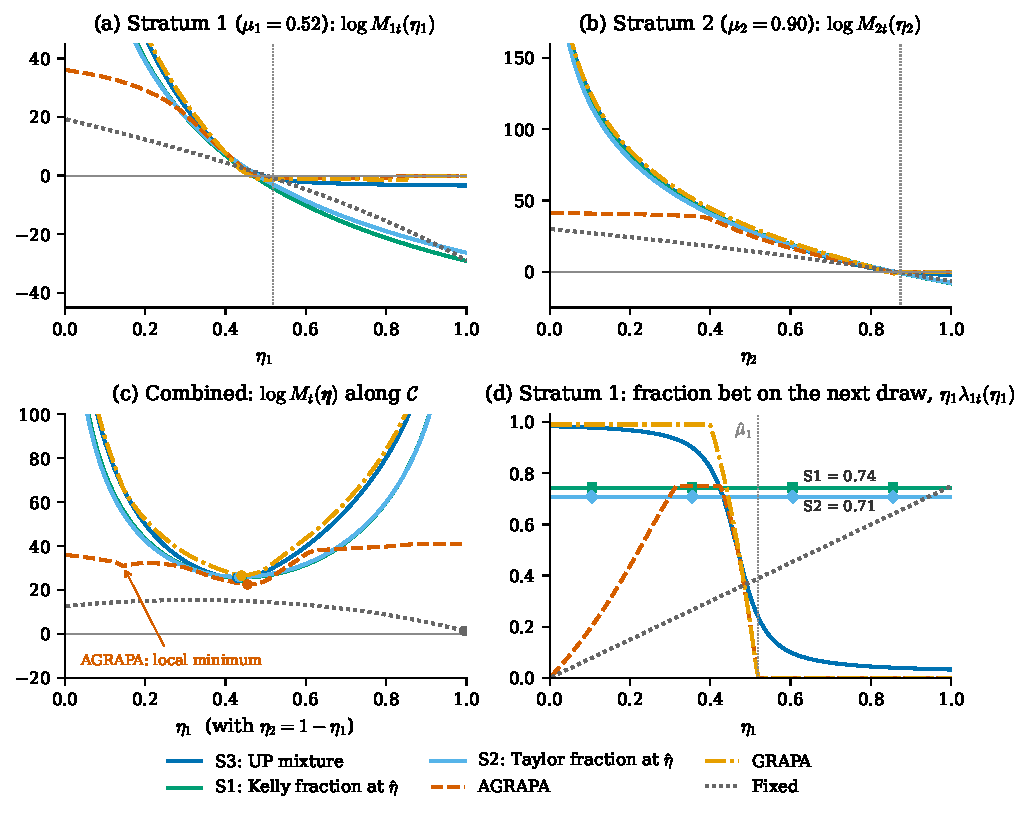
\includegraphics[width=\textwidth]{figures/fig_k2_anatomy.pdf}
  \caption{One UI-TS with $K=2$, $w_k=1/2$, $\eta_0=1/2$, after $n_k=60$ round-robin draws from strata with means
  $0.52$ and $0.90$.  Solid lines are convexifying bets; broken lines are not.  (a, b) Stratum log-wealth
  $\log M_{kt}(\eta_k)$; dotted vertical lines mark the sample means.  (c) The objective $\log M_t(\bs\eta)$ along $\calC$;
  dots mark minima.  (d) The fraction of wealth each rule would bet on the next draw from stratum 1, as a function of
  the null.  The S1 and S2 fractions do not depend on the null ($0.74$ and $0.71$ here); in stratum 2, both sit at the cap
  $\cbar=0.9$.}
  \label{fig:anatomy}
\end{figure}

\paragraph{Three strata at a fixed sample size.}  \Cref{tab:uits} reports, for $K=3$ strata with equal weights,
$\eta_0=1/2$ and $\bs\mu=(0.58,0.64,0.72)$, the UI-TS after $n_k$ draws per stratum.  S1 essentially matches GRAPA
(medians \kellyrefKthree{} and \grapaKthree{} at $n_k=100$), as \cref{thm:nocost} suggests, and S2 and S3 are close
behind (\taylorrefKthree{} and \upKthree{}), all ahead of AGRAPA (\agrapaKthree{}).  For the rules that are not
convexifying, these values are the exact minima over the lattice; a local search from $(1/2,1/2,1/2)$ missed AGRAPA's
global minimum by more than $0.05$ in \agrapamissshare{} of runs at $n_k=30$, and never missed for the convexifying rules.

\begin{table}[t]
  \centering\small
  \caption{$K=3$, $w_k=1/3$, $\eta_0=1/2$, $\bs\mu=(0.58,0.64,0.72)$, \repsB{} replications: median of
  $\min_{\bs\eta\in\calC}\log M_t(\bs\eta)$ after $n_k$ round-robin draws per stratum.}
  \label{tab:uits}
  \begin{tabular}{llrr}
\toprule
 & & \multicolumn{2}{c}{median $\log M_t$}\\
\cmidrule(lr){3-4}
Bet & Class & $n_k=30$ & $n_k=100$\\
\midrule
S1: Kelly fraction at $\hat{\boldsymbol\eta}$ & convexifying & 14.9 & 49.3\\
S2: Taylor fraction at $\hat{\boldsymbol\eta}$ & convexifying & 13.8 & 48.5\\
S3: UP mixture & convexifying & 12.8 & 46.6\\
\addlinespace
Fixed & concavifying & 3.2 & 10.1\\
Binary Kelly & neither & 6.2 & 21.2\\
ST-Bern (ALPHA) & neither & 9.3 & 26.7\\
AGRAPA & neither & 12.1 & 43.6\\
GRAPA & neither & 13.9 & 49.8\\
\bottomrule
\end{tabular}

\end{table}

\paragraph{Stopping times.}  \Cref{fig:stopping} reports the expected number of draws until the UI-TS reaches $1/\alpha$
($\alpha=5\%$), in the style of \citet[Figure 3]{spertus2024sequential}, for $K=2$, $w_k=1/2$, $\eta_0=1/2$, and Beta
strata with global mean $\mu$ and stratum means either equal or $\mu\mp0.2$.  S1 stopped sooner than AGRAPA in every
design, by \fkellyvsagrapamin{} to \fkellyvsagrapamax{}, and S3 by \fupvsagrapamin{} to \fupvsagrapamax{}.  S2 is the
least consistent of the three: it is close to S1 when the alternative is near the null, where its quadratic
approximation is accurate, but it can need up to \ftaylorvskellymax{} more draws than S1 when the optimal fraction is
large.  Fixed bets are left out of the figure because they perform terribly: at $\mu=0.6$ with equal stratum means
they needed \ffixedtau{} draws on average, against \fkellytau{} for S1, and hit the $3000$-draw cap in \ffixedcens{} of runs;
with stratum means $0.4$ and $0.8$ they hit it in \ffixedgapcens{} of runs.  The reason is that their minimum is at a
vertex of $\calC$, where the I-TSM at $(1,0)$ has negative expected log-growth.  GRAPA is omitted because recomputing its bets at every null after every draw is slow.

\begin{figure}[tbp]
  \centering
  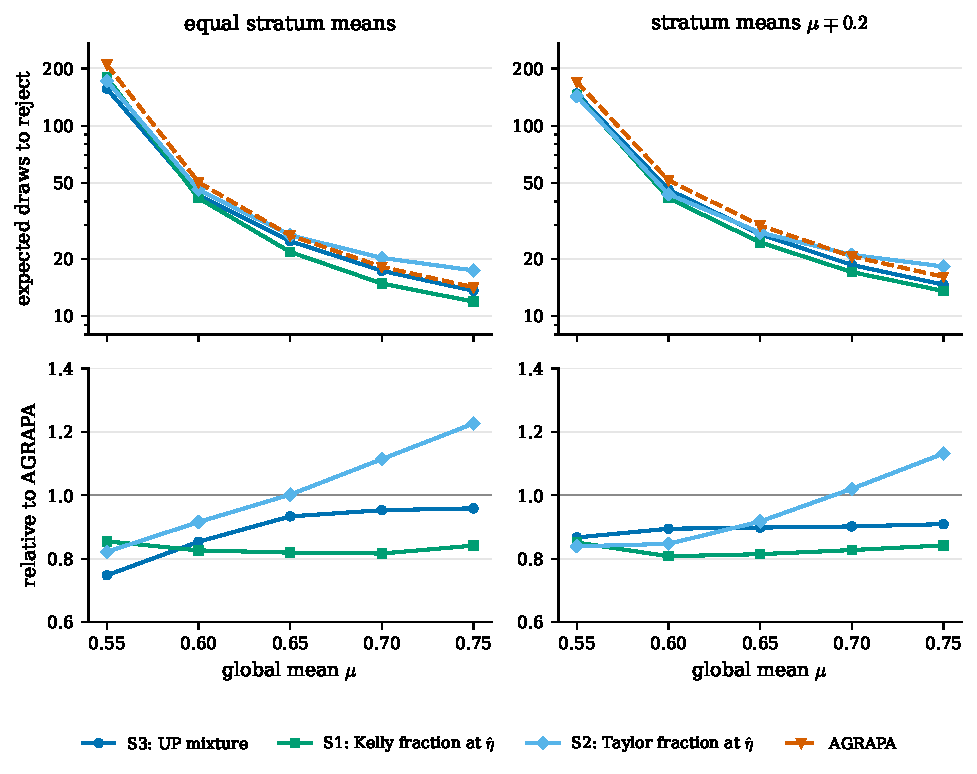
\includegraphics[width=\textwidth]{figures/fig_stopping_beta.pdf}
  \caption{Top: expected number of draws (log scale) until the UI-TS rejects $H_0:\mu\le1/2$ at level $5\%$, for $K=2$,
  $w_k=1/2$, round-robin selection, and Beta strata with global mean $\mu$; \repsF{} replications per point.  Runs are
  capped at $3000$ draws, a cap that none of the rules shown ever reached; fixed bets, which often did, are omitted (see
  the text).  Bottom:
  the same expectations divided by AGRAPA's; values below $1$ mean fewer draws than AGRAPA.  Solid lines are convexifying
  bets.}
  \label{fig:stopping}
\end{figure}

\paragraph{Perfect stratification.}  Stratification helps most when the strata are homogeneous.
Following \citet[Figure 5]{spertus2024sequential}, \cref{fig:twopoint} considers a population with two support points,
$\mu\mp\delta/2$, in equal proportions, so that $\delta$ is the spread between the points.  Under perfect stratification,
each stratum contains one of the points ($K=2$, $w_k=1/2$); the stratified UI-TS with S3 is compared with the
unstratified UP TSM, which samples the two-point population at random and tests $\mu\le1/2$ directly.  The stratified
test barely sees the spread: for $\mu=0.55$ its expected stopping time grows from \hstratAzero{} draws at $\delta=0$ to
\hstratAmax{} at $\delta=0.8$, while the unstratified test needs \hunstratAmax{} at $\delta=0.8$, \hratioAup{} times as many
(\hratioAkelly{} times with Kelly-type bets, S1 against the GRAPA TSM).  For $\mu=0.6$ the ratio at $\delta=0.8$ is
\hratioBup{} (\hratioBkelly{} with Kelly-type bets).  Far from the null both tests stop within about $20$ draws and the
ratio stays below \hratioCmax{}.  With little spread there is nothing to gain from stratifying, and the UI-TS pays a small
price for taking the minimum over $\calC$: at $\delta=0$ the unstratified test is slightly faster (ratio \hratiozero{}).

\begin{figure}[tbp]
  \centering
  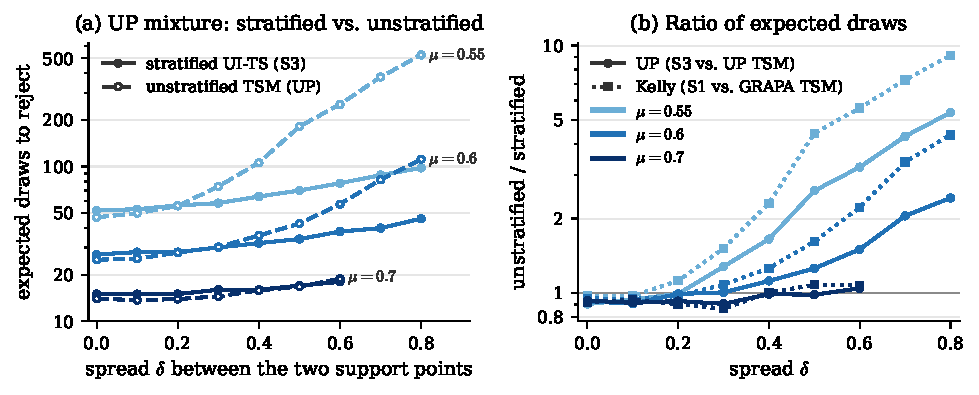
\includegraphics[width=\textwidth]{figures/fig_two_point.pdf}
  \caption{Perfect stratification of a two-point population with support $\mu\mp\delta/2$ in equal proportions, testing
  $\mu\le1/2$ at level $5\%$.  (a) Expected draws to reject (log scale) for the stratified UI-TS with S3 (solid; the data
  are deterministic, so one run) and for the unstratified UP TSM (dashed; \repsH{} replications).  (b) The ratio of
  unstratified to stratified expected draws, for UP (S3 against the UP TSM) and for Kelly-type bets (S1 against the
  GRAPA TSM, $200$ replications).}
  \label{fig:twopoint}
\end{figure}

\paragraph{Selection.}  \Cref{tab:selection} compares round robin, the greedy rule \eqref{eq:greedy}, and the oracle
allocation that tracks $\bs p^\star$ (computed from the true distributions), for $K=2$, $w_k=1/2$, $\eta_0=1/2$ and three
designs: different means, where round robin happens to be optimal ($p^\star_1=\pstarA$); equal means and different
spreads ($p^\star_1=\pstarB$), where the noisier stratum should be sampled more; and one stratum far below the null and
one far above it ($p^\star_1=\pstarC$), where the stratum above the null should be sampled more.  Where the allocation
matters, the greedy rule moved the proportions towards $\bs p^\star$ and reduced the expected number of draws by
\iselgainmin{} to \iselgainmax{} relative to round robin.  It needed at most \iselvsoraclemax{} more draws than the oracle,
and fewer in \iselbeatoracle{} of the four cases, presumably because it adapts to the realized data while the oracle
tracks the asymptotic proportions.  Where round robin is optimal, the greedy rule was within \iselmeansdiff{} of it,
which is within simulation error.

\begin{table}[t]
  \centering\small
  \caption{Selection rules for $K=2$, $w_k=1/2$, $\eta_0=1/2$, \repsI{} replications; strata are
  $\mathrm{Beta}(\kappa\mu_k,\kappa(1-\mu_k))$ with the means $\mu_k$ and concentrations $\kappa$ shown.  Expected number of draws
  to reject at level $5\%$, and the average share of draws taken from stratum 1.  Oracle: deterministic allocation
  tracking the optimal proportions $\bs p^\star$.}
  \label{tab:selection}
  \begin{tabular}{llrrrrrr}
\toprule
 & & \multicolumn{3}{c}{expected draws} & \multicolumn{3}{c}{share of draws from stratum 1}\\
\cmidrule(lr){3-5}\cmidrule(lr){6-8}
$(\mu_1,\kappa_1)$, $(\mu_2,\kappa_2)$ & Bet & round robin & greedy & oracle & round robin & greedy & oracle\\
\midrule
(0.4, 4), (0.7, 4) & S1 & 157 & 162 & 157 & 0.50 & 0.48 & 0.50\\
 & S3 & 151 & 146 & 151 & 0.50 & 0.46 & 0.50\\
\addlinespace
(0.55, 2), (0.55, 100) & S1 & 145 & 118 & 119 & 0.51 & 0.66 & 0.65\\
 & S3 & 131 & 122 & 126 & 0.51 & 0.63 & 0.65\\
\addlinespace
(0.2, 4), (0.95, 4) & S1 & 56 & 48 & 51 & 0.51 & 0.36 & 0.28\\
 & S3 & 77 & 59 & 55 & 0.50 & 0.32 & 0.28\\
\bottomrule
\end{tabular}

\end{table}

\paragraph{Implementation check.}  The product of the predictable UP bets $\lambda^{\up}_{ki}=\hat c_{ki}/\eta_k$ equals the
mixture \eqref{eq:up} exactly, which makes a useful unit test.  Applied to the repository's
\texttt{Bets.universal\_portfolio}, it shows that the bet for observation $i$ there uses observations $1,\ldots,i$ rather
than $1,\ldots,i-1$; shifting it by one restores predictability and the identity (see \texttt{code/test\_against\_repo.py}).

% ============================================================================================
\section{Discussion and open questions}\label{sec:discussion}
% ============================================================================================

\paragraph{Summary.}  Convexity of the UI-TS is governed by two scalar functions per betting rule, the payoffs on the
extreme outcomes.  Every fraction of wealth that does not depend on the null is convexifying, and the best such
fraction, Kelly at the least-favorable null, grows as fast as betting Kelly separately at every null.  Truncation, the
standard device for adaptive bets, is exactly what excludes most rules in use.  The three strategies of
\cref{sec:strategies} make each step of the UI-TS a smooth convex program, solved by water-filling in time linear in
the number of draws, without giving up efficiency: in our simulations the predictable Kelly fraction at the estimated
least-favorable null stopped sooner than AGRAPA in every design and was the fastest rule in \fsonebest{} of the
\fndesigns{} designs.

\paragraph{Open questions.}
\begin{enumerate}
  \item \emph{Consistency of the plug-in.}  Does the estimated least-favorable null converge to $\bs\eta^\star$ when the
  fractions are themselves estimated at it (S1, S2), so that S1 attains the rate $\gamma^\star$ without oracle knowledge?
  Does greedy selection converge to $\bs p^\star$, as upper-confidence Frank--Wolfe does for smooth objectives?
  \item \emph{Sampling without replacement.}  Without replacement, the stratum null is updated to $\eta_{kt}$, an
  increasing affine function of $\eta_k$.  If the bet is a convexifying rule evaluated at $\eta_{kt}$, the factor is
  log-convex in $\eta_k$ (composition with an affine map).  The repository instead evaluates bets at $\eta_k$ while
  centering at $\eta_{kt}$, which \cref{thm:characterization} does not cover.  \todo{Characterize this case.}
  \item \emph{The concave case with many strata.}  For arbitrary concave stratumwise functions and unequal weights,
  minimizing $\sum_kL_k(\eta_k)$ over $\calC$ (equivalently, over its vertices) is NP-hard: with $L_k(\eta)=\eta(1-\eta)$
  the minimum is $0$ iff some vertex is integral, which is subset sum \citep{garey1979computers}.  With equal weights,
  every vertex has $m\in\{\lceil K\eta_0\rceil-1,\lfloor K\eta_0\rfloor\}$ coordinates at $1$, at most one fractional
  coordinate, and the rest at $0$, so the minimum can be found in $O(K^2\log K)$ time by choosing the fractional
  coordinate and then the $m$ strata with the smallest $L_k(1)-L_k(0)$.
  \item \emph{Connection to the Gaffke--bootstrap--EL--betting chain.}  \Cref{app:regret} places the UP UI-TS between
  stratified empirical likelihood and anytime-valid betting, with an explicit price for predictability.  How does it
  compare with a stratified Gaffke bound at a fixed sample size?
\end{enumerate}

\bibliographystyle{plainnat}
\bibliography{refs}

% ============================================================================================
\appendix
\section{Convexifying arbitrary stratumwise bets}\label{app:convexify}
% ============================================================================================

When the bets are not convexifying, a convex lower bound on the objective still gives a valid test, since a valid
UI-TS only needs to be bounded above by the I-TSM at the true intersection null.  Let $\conv L_k$ be the largest convex
function below $L_{kt}$ on $[0,1]$ (its convex envelope), and $\rho_k := \sup_{\eta}[L_{kt}(\eta)-\conv L_k(\eta)]$ its
nonconvexity.

\begin{proposition}\label{prop:convexify}
Under \cref{ass:separable}, with each $L_{kt}$ lower semicontinuous, let
$\log\conv M_t := \min_{\bs\eta\in\calC}\sum_k\conv L_k(\eta_k)$ and $\log\underline M_t := \min_{\bs\eta\in\calC}\sum_kL_{kt}(\eta_k)$.
Then $\max_{j\le t}\conv M_j$ is a valid UI-TS computable by convex optimization, and
$0\le\log\underline M_t-\log\conv M_t\le\max_k\rho_k$.
\end{proposition}

\begin{proof}[Proof sketch]
Validity: $\conv M_j$ is at most the I-TSM at any point of $\calC$, in particular at the true intersection null.  For the
gap, at a minimizer $\breve{\bs\eta}$ of the convexified problem each $\conv L_k$ is either equal to $L_{kt}$ or affine on
an interval $[a_k,b_k]\ni\breve\eta_k$ with equality at the endpoints \citep[Section 17]{rockafellar1970convex}.  Minimizing
the (now affine) objective over $\{\bs\eta\in\prod_k[a_k,b_k]:\bs w\cdot\bs\eta=\eta_0\}$ has an optimal vertex with at most
one coordinate strictly inside its interval; at every other coordinate $L_{kt}=\conv L_k$.  This is a one-constraint
version of the Shapley--Folkman duality-gap bound \citep{starr1969quasi, aubin1976estimates}.
\end{proof}

In the design of \cref{tab:uits} with $n_k=100$, convexifying GRAPA this way cost at most \grapaconvloss{} in log-wealth
(95th percentile), but convexifying AGRAPA cost \agrapaconvloss{}, because its curves are concave over a wide range.  On a
grid, the envelope must also be kept below $L_{kt}$ between grid points to preserve validity.  We have not pursued this
further, because the strategies of \cref{sec:strategies} are convex by construction and at least as efficient.

% ============================================================================================
\section{The mixture strategy and stratified empirical likelihood}\label{app:regret}
% ============================================================================================

\begin{proposition}[Regret of the UP mixture]\label{prop:regret}
Each $\log M^{\mix}_{kt}$ is convex, nonincreasing, and smooth on $(0,1]$.  With $n_k := T_k(t)$ and $\ell_{n_k}$ the
hindsight log-wealth \eqref{eq:el} of stratum $k$, for every $\bs\eta$,
\begin{gather*}
\sum_{k=1}^K \ell_{n_k}(\eta_k) - R_t \;\le\; \log\prod_{k=1}^K M^{\mix}_{kt}(\eta_k) \;\le\; \sum_{k=1}^K \ell_{n_k}(\eta_k),\\
R_t = \begin{cases}\sum_k\log(n_k+1) & \pi=\mathrm{Uniform}(0,1),\\[2pt]
\sum_k\bigl[\tfrac12\log(n_k+1)+\log2\bigr] & \pi=\mathrm{Beta}(1/2,1/2),\end{cases}
\end{gather*}
so $\min_{\bs\eta\in\calC}\log\prod_k M^{\mix}_{kt}(\eta_k)$ is within $R_t$ of $\min_{\bs\eta\in\calC}\sum_k\ell_{n_k}(\eta_k)$.
\end{proposition}

\begin{proof}
Each factor $1-c+cX/\eta$ is nonincreasing in $\eta$, hence so is the mixture, and smoothness follows from
differentiating under the integral; convexity is \cref{prop:closure}(ii).  The integrand is the wealth of a
constant-rebalanced portfolio, so the mixture is at most the best such wealth, $\exp\ell_{n_k}(\eta_k)$.  For the lower
bound, the universal portfolio with a uniform (respectively Dirichlet$(1/2,1/2)$) prior has wealth at least that of the
best constant-rebalanced portfolio in hindsight divided by $n+1$ (respectively by $2\sqrt{n+1}$) for every sequence of
nonnegative returns \citep{cover1996universal}.  Sum over strata; the bounds pass to the minima over $\calC$ because they
hold for every $\bs\eta$.
\end{proof}

The quantity $\min_{\bs\eta}\sum_k\ell_{n_k}(\eta_k)$ is a stratified, one-sided empirical-likelihood statistic
\citep[cf.][]{owen1988empirical}, itself a convex program by \cref{ex:el}.  So S3 is a predictable, anytime-valid version of
stratified empirical likelihood, at a price of at most $R_t$ in log-wealth.  Because $\ell_{n_k}(\eta_k)$ is at least the
log-wealth of the constant fraction $c^\star_k$ of \cref{thm:nocost}(ii), and $R_t/t\to0$, the argument for
\cref{thm:nocost}(ii) shows that $\liminf_t t^{-1}\min_{\bs\eta}\log\prod_kM^{\mix}_{kt}(\eta_k)\ge\gamma^\star$ almost surely: S3
grows at least as fast as the best UI-TS with fractions capped at $\cbar$, without knowing $\bs\eta^\star$.

\end{document}
